\documentclass[11pt]{book}
\usepackage{fontspec}
\usepackage{yeban-manual}
\title{Yeban User Guide}
\author{Yeban}
\date{}
\begin{document}
\maketitle
\tableofcontents
% Yeban User Guide — Chapter 1 sample (English)
% T-DOC-001 first package. Section-by-section counterpart of the Chinese sample.
% Sources: README.md, docs/manual/01-overview.md, 02-projects.md,
% crates/yeban-app/src/help.rs, crates/yeban-app/src/cli.rs SHORTCUTS.

\chapter{Getting Started}
\label{ch:quickstart}

\classquote{不积跬步，无以至千里。}{Xunzi, “Encouraging Learning” (《荀子·劝学》)}{Translation: “Without accumulating small steps, one cannot reach a thousand li.” This chapter takes you from installation to your first export, one step at a time: make sound first, refine later.}





Yeban is an open-source digital audio workstation: a pure-Rust, low-latency real-time
audio engine with a native Slint GUI and a complete MCP tool surface. A human at the
desktop and an AI agent can work on the same project side by side. This chapter takes
you from installation to your first export, using only features that actually exist.

\section{Installation and First Launch}

\subsection{Choose an installation method}

The easiest route is the nightly installers in the Download table of \texttt{README.md}
(they track \texttt{main} and are unsigned): an MSI for Windows x86\_64, DMG images for
macOS (Apple Silicon and Intel), and DEB packages for Linux (x86\_64 and arm64).
Portable \texttt{.tar.gz} archives and \texttt{SHA256SUMS} are on the nightly release page.

\paragraph{Building from source} requires Rust 1.99.0 (pinned by
\texttt{rust-toolchain.toml}; \texttt{rustup} installs it automatically), a C++
compiler and \texttt{libclang} (\texttt{yeban-dsp} generates bindings with bindgen).
On Ubuntu/Debian:

\begin{verbatim}
sudo apt-get install -y clang libclang-dev pkg-config libfontconfig1-dev \
  libfreetype-dev libxkbcommon-dev libxkbcommon-x11-0 libwayland-dev \
  libx11-dev libgl1-mesa-dev libasound2-dev
cargo build --release -p yeban-app
\end{verbatim}

Run it with \texttt{cargo run --release -p yeban-app}; add \texttt{-- --headless} on a
machine without a display. On a memory-tight machine, build with
\texttt{cargo build --profile release-small -p yeban-app}.

\begin{figure}[htbp]
\centering
\begin{tikzpicture}[node distance=0.45cm, >=stealth,
    box/.style={draw, rounded corners, align=center, font=\small, minimum width=2.0cm, minimum height=0.8cm}]
  \node[box] (a) {Installer / build};
  \node[box, right=of a] (b) {First launch};
  \node[box, right=of b] (c) {Onboarding tour};
  \node[box, right=of c] (d) {Track + clip};
  \node[box, right=of d] (e) {Audition};
  \node[box, right=of e] (f) {Export WAV};
  \draw[->] (a) -- (b); \draw[->] (b) -- (c); \draw[->] (c) -- (d);
  \draw[->] (d) -- (e); \draw[->] (e) -- (f);
\end{tikzpicture}
\caption{The hands-on route: install $\to$ launch $\to$ tour $\to$ arrange $\to$ audition $\to$ export}
\label{fig:ch01-flow}
\end{figure}

\subsection{First launch and the onboarding tour}

On first launch the app automatically opens the onboarding tour (only when persisted
state says it should: it will not reopen once dismissed with ``don't show again'' or
completed). The tour walks through the welcome page, transport bar, arrangement area,
piano roll and mixer console, ending with the inspector and sound library. Each step
navigates the interface to the area it describes. To see it again, use Help $\to$
Onboarding Tour.

\screenshot{ch01-onboarding-tour}{The onboarding card on first launch, stopped at the ``transport bar'' step}

\section{Interface Overview}

\subsection{Menu bar and transport bar}

The menu bar has eight groups: File, Edit, Track, Transport, Mix, View, Diagnostics
and Help. The transport bar at the top has play/pause (Space), stop, return to
\texttt{001.01.000}, cycle toggle (C), metronome and count-in, plus the tempo (BPM)
display and tap input. On its right is the workspace switcher: Overview, Live Launch,
Linear Arrangement and Mixer Console, mapped to number keys 1--4.

\screenshot{ch01-main-window}{The main window with the built-in demo project open, labelling the menu bar, transport bar, arrangement area, inspector and bottom console}

\subsection{Centre: the arrangement area}

Each track is a row: the left part is the track header (name, mute/solo, volume), and
clips sit on the timeline to its right. Clips can be dragged, resized by their edges,
copied (Cmd/Ctrl+C / Cmd/Ctrl+V), cut (Cmd/Ctrl+X) and deleted. Above are the bar ruler
and section markers; below you can expand the chord track and automation lanes. Press
Tab to open the Clip Launch Matrix (Session view) and fire clips from its grid.

\subsection{Left: inspector and sound library}

The upper-left pane is the channel inspector, showing the selected track's channel
strip and device parameters; I toggles it. The lower-left pane is the sound library,
where you browse presets and SFZ libraries. The first button in the track-header tool
row is the Track Menu, collecting all operations for that track.

\subsection{Bottom console and edges}

Three bottom tabs: piano roll (P / F7), mixer console (X / F8) and device rack (F9);
F3 maximises/restores the console. On the right you can open the Control Room (F4),
showing master monitoring and loudness readings. The status bar at the bottom shows
selection info, live chord recognition, shortcut hints and audio-device status; below
it is the song-overview panel. Hovering over a control shows a tooltip; T toggles them.

\begin{table}[htbp]
\centering
\caption{Keys used in this chapter (canonical labels; Cmd+ on macOS, Ctrl+ elsewhere)}
\label{tab:ch01-keys}
\begin{tabular}{ll}
\hline
Key & Action \\
\hline
Space & Play / pause \\
Shift+Space & Resume from cursor \\
C & Cycle playback toggle \\
Enter & Return to start \\
Tab / F5 & View switch / Session view \\
F6 & Arrangement view \\
P / F7 & Piano roll \\
X / F8 & Mixer console \\
F9 & Device rack \\
I & Toggle left inspector \\
Cmd/Ctrl+S & Save project \\
Cmd/Ctrl+Shift+S & Save as \\
Cmd/Ctrl+Z / Cmd/Ctrl+Shift+Z & Undo / redo \\
Cmd/Ctrl+T & Split selected clip at playhead \\
\hline
\end{tabular}
\end{table}

\section{Your First Project}

\subsection{Start empty, or tour the demo first}

A project uses the \texttt{.yeban} extension and is the only project format: one
container holds tracks, clips, notes, device chains and the assets they use.

File $\to$ New Empty Project gives you a project with only the master bus. If you
launch without specifying a project, the app opens a demo project (drums, bass, pad,
lead, strings, percussion) so you can look around first; it is not your work file, so
editing it cannot lose anything of yours.

\subsection{Create a track, place a clip, play}

In an empty project, create an audio track from the Track Menu; pick a preset or SFZ
instrument in the sound library and place an audio clip on the timeline. Press Space to
play — the transport shows position and tempo. To loop a passage, press C and select a
range. If a clip lands in the wrong place, drag it or drag its edge to resize; to split
it at the playhead, select it and press Cmd/Ctrl+T.

\screenshot{ch01-first-clip}{A clip placed on track 1 of an empty project, with the playhead in the middle of the clip}

\subsection{Save and export}

File $\to$ Save Project (Cmd/Ctrl+S) writes back to the original file;
File $\to$ Save As (Cmd/Ctrl+Shift+S) changes the name or location. Saving is atomic,
so a power cut mid-write cannot leave a half-written file.

Full-mix WAV export lives in the File menu. Stem export renders each source-node track
into a 32-bit Float WAV in a fixed output directory, and produces a
\texttt{stems-manifest.json} index plus a one-line export receipt. The master bus
produces no file but is named in the skipped list — that is not a dropped track.

\screenshot{ch01-export-dialog}{The export dialog and the resulting receipt/toast message}

\section{Help Topic Mapping}

\begin{table}[htbp]
\centering
\caption{Sections of this chapter $\to$ in-app help anchors}
\label{tab:ch01-help}
\begin{tabular}{ll}
\hline
Section & Help topic \\
\hline
Installation and first launch & \texttt{getting-started-install} \\
Onboarding tour & \texttt{getting-started-onboarding} \\
Menu bar and transport bar & \texttt{interface-transport} \\
Arrangement area & \texttt{interface-arrangement} \\
Inspector and sound library & \texttt{interface-inspector-library} \\
Bottom console and edges & \texttt{interface-console} \\
New project / demo project & \texttt{project-new-demo} \\
Track, clip and playback & \texttt{project-first-arrange} \\
Save and export & \texttt{project-save-export} \\
\hline
\end{tabular}
\end{table}

\paragraph{What you will be able to do} Complete the whole flow — install, launch, create a track, place a clip, play back and export — and name the five main interface areas.

\paragraph{Hands-on exercise} Create an empty project, place one demo audio clip on track 1; press Space to play and C to loop two bars; save with Cmd/Ctrl+S; export a full-mix WAV and a stem set; finally reopen via File $\to$ Open / Restore and verify the clip is still there.

% Yeban User Guide — Chapter 2: Projects (English)
% T-DOC-001 chapter-by-chapter delivery. Same structure as the Chinese chapter.
% Sources: app.slint menus, host.rs project/template/chooser wiring,
% startup_chooser.rs NewProjectDetails, docs/manual/02-projects.md.

\chapter{Projects}
\label{ch:projects}

This chapter covers the whole project lifecycle: how to create, open, save and reuse
a project, plus Yeban's distinctive "undo is versioning" model. By the end you should
be able to save work confidently, find it again, and return to any past state.

\section{Create, Open and Save}

\subsection{Five entries in the File menu}

The File menu has five project-related items:

\begin{itemize}
  \item \textbf{New Empty Project}: a project with only the master bus.
  \item \textbf{New from Template...}: opens the template chooser to start from a factory or user template.
  \item \textbf{Open / Restore Project...}: pick a \texttt{.yeban} file in the file dialog.
  \item \textbf{Save Project (Cmd/Ctrl+S)}: write the current project back to its file.
  \item \textbf{Save As (Cmd/Ctrl+Shift+S)}: save under a different name or location.
\end{itemize}

You can also open directly from the command line: \texttt{yeban-app --open <path>}.

\screenshot{ch02-file-menu}{The File menu expanded, labelling New Empty Project, New from Template, Open/Restore, Save and Save As}

\subsection{The startup project chooser}

When you launch without specifying a project, the startup project chooser appears.
It groups entry points into \textbf{Recent Projects}, \textbf{Demo Projects},
\textbf{Factory Templates}, \textbf{User Templates}, and an empty-project entry left
on the ``New Project'' tab. A demo lets you look around without touching your work;
a recent project returns you to where you left off.

\screenshot{ch02-startup-chooser}{The startup project chooser with its four category tabs and the ``New Project'' tab}

\subsection{Saving is atomic}

Saving is atomic: content is written to a temporary location first and replaces the
target only once it is complete. A power cut mid-write cannot leave a half-written
project — you get either the new version or the previous one.

\begin{figure}[htbp]
\centering
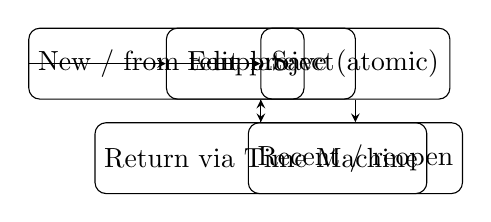
\begin{tikzpicture}[node distance=1.2cm, >=stealth,
    box/.style={draw, rounded corners, align=center, minimum width=2.4cm, minimum height=0.9cm}]
  \node[box] (a) {New / from template};
  \node[box, right of=a] (b) {Edit project};
  \node[box, right of=b] (c) {Save (atomic)};
  \node[box, below of=c] (d) {Recent / reopen};
  \node[box, below of=b] (e) {Return via Time Machine};
  \draw[->] (a) -- (b); \draw[->] (b) -- (c); \draw[->] (c) -- (d);
  \draw[->] (b) -- (e); \draw[->] (e) -- (b);
\end{tikzpicture}
\caption{Project lifecycle: new/from template $\to$ edit $\to$ save $\to$ reopen; you can return to an older version at any time}
\label{fig:ch02-lifecycle}
\end{figure}

\section{Project Files and the Asset Pool}

A project uses the \texttt{.yeban} extension and is the only project format. One
container holds tracks, clips, notes, device chains, and the materials the project
uses (kept in the asset pool, addressed by content hash).

The asset pool means "the project brings its own materials": copy a project to
another machine and the audio and SFZ samples it uses travel with the container.
Stem export and Save As Template both take the pool from the same source, matching
the CLI and MCP behaviour (see Chapter 8).

\begin{table}[htbp]
\centering
\caption{Where things live inside a project}
\label{tab:ch02-container}
\begin{tabular}{ll}
\hline
Content & Location in the project \\
\hline
Tracks / clips / notes & Arrangement data \\
Device chains & The device sequence of each track \\
History DAG & The undo chain, saved with the project \\
Used materials & Asset pool, addressed by content hash \\
Project settings & Tempo / key / time signature / sample rate \\
\hline
\end{tabular}
\end{table}

\section{Templates: New from Template, Save As, Factory Directory}

\subsection{New from template}

File $\to$ New from Template... opens the template chooser, listing two kinds:
\textbf{factory templates} (shipped with the app) and \textbf{user templates} (ones
you saved). Selecting one creates a new project from that skeleton. When the list is
long, the chooser reports the number of hidden rows rather than silently dropping
entries.

\subsection{Save as template}

File $\to$ Save As Template... opens a dialog: enter a name, then confirm to write
into the user template directory. If a template with that name already exists, the
app does not overwrite it directly — it stops and asks for confirmation; cancelling
writes nothing. The user template directory is created on first use; if it is
unavailable, the dialog shows the error rather than failing silently.

\screenshot{ch02-template-dialog}{The Save As Template dialog showing the name field, hint line and same-name confirmation state}

\section{Recent Projects and Recovery}

Every successful open records the path in Recent Projects. You find it under the
``Recent Projects'' tab of the startup chooser and open it with one click; the list
also offers a removal entry for records you no longer need. Recent projects, language
and layout share one local settings store, so changing language or layout does not
push recent projects out.

Open / Restore Project... is also used for recovery: after you select a container
file, the app restores the scene from the history DAG and asset pool recorded in it.

\section{Project Settings: Sample Rate, Tempo, Time Signature}

On the ``New Project'' tab of the startup chooser you can set a few basics for the
empty project; they are written into the new project:

\begin{itemize}
  \item \textbf{Tempo (BPM)}: accepted range 20--999; out-of-range or invalid input is folded back into the legal domain.
  \item \textbf{Key signature}: it can be unset (the factory state of a canonical empty project), or use sharps/flats from $-7$ to $+7$.
  \item \textbf{Time signature}: numerator 1--32; denominator only 1, 2, 4, 8, 16 or 32.
  \item \textbf{Sample rate}: the project's audio sample rate (Hz).
\end{itemize}

These drive later conversions: bar length comes from the time signature, and the
timecode grid from the project's time signature. When a time signature is invalid,
the app reports the reason literally (e.g.\ ``invalid time signature, cannot compute
clip length'') instead of quietly substituting a default.

\screenshot{ch02-new-project-details}{The New Project tab showing the four inputs: tempo, key signature, time signature and sample rate}

\section{Undo Is Versioning: the Time Machine}

Yeban has no separate "version history" feature: every edit is a commit, and undo/
redo merely move along that commit chain.

\begin{itemize}
  \item \textbf{Undo}: Cmd/Ctrl+Z; \textbf{Redo}: Cmd/Ctrl+Shift+Z.
  \item \textbf{Time Machine (Undo Tree)}: Edit $\to$ Time Machine (Undo Tree)...; Cmd/Ctrl+Shift+H also opens it.
\end{itemize}

The Time Machine draws the whole commit chain as a graph: click any version node to
return the project to that state. If there are too many older versions to fit, the
panel reports how many were not drawn rather than pretending all are shown. The
history DAG is saved with the project, so it is still there next time you open it.

\screenshot{ch02-undo-tree}{The Undo Tree graph with a historical node selected and highlighted}

\section{Help Topic Mapping}

\begin{table}[htbp]
\centering
\caption{Sections of this chapter $\to$ in-app help anchors}
\label{tab:ch02-help}
\begin{tabular}{ll}
\hline
Section & Help topic \\
\hline
Five entries in the File menu & \texttt{project-file-menu} \\
Startup project chooser & \texttt{project-startup-chooser} \\
Saving is atomic & \texttt{project-atomic-save} \\
Project files and asset pool & \texttt{project-container-assets} \\
New from template & \texttt{project-template-new} \\
Save as template & \texttt{project-template-save} \\
Recent projects and recovery & \texttt{project-recent-recovery} \\
Project settings & \texttt{project-settings} \\
Undo is versioning: Time Machine & \texttt{project-undo-tree} \\
\hline
\end{tabular}
\end{table}

\paragraph{What you will be able to do} Create, open, save and reuse a project, return to any historical version with the Time Machine, and explain what a \texttt{.yeban} container holds.

\paragraph{Hands-on exercise} Create a project from a template, set tempo to 96 BPM and time signature 3/4; save it, then save it as a template; make several edits, undo with Cmd/Ctrl+Z and jump back to the earliest version with the Time Machine; finally quit, reopen from Recent Projects in the startup chooser and verify the settings survived.

% Yeban User Guide — Chapter 3: Tracks and Clips (English)
% T-DOC-001 chapter-by-chapter delivery, written ahead of the CH03 task.
% Sources: app.slint menus and clip-drag callbacks, cli.rs SHORTCUTS, docs/manual/01-overview.md.

\chapter{Tracks and Clips}
\label{ch:tracks-clips}

\begin{quote}
方以类聚，物以群分。
\end{quote}

Source: Book of Changes, “Appended Judgments I” (《周易·系辞上》). Translation: “Things gather according to their kind; creatures divide according to their group.”

Tracks and clips find their place by kind; clear grouping is what makes editing orderly.

The arrangement area is Yeban's main workspace: tracks as rows, clips laid out on the
timeline to their right. This chapter covers creating tracks, placing clips and turning
a piece of material into the arrangement you want.

\section{Track Types and the Track Header}

\subsection{Three track types}

The Track menu offers three creation entries:

\begin{itemize}
  \item \textbf{New MIDI Synth Track (Cmd/Ctrl+N)}: sounds via a built-in synthesizer or plugin instrument, holding MIDI clips.
  \item \textbf{New Audio Track}: holds recorded or imported audio clips.
  \item \textbf{New Aux Bus Track}: receives sends from other tracks for summing and group processing.
\end{itemize}

Delete Selected Track removes the selected track from the menu.

\subsection{The track header}

Each track's left side is the header: name, mute/solo switches, volume, and the Track
Menu button at the very front (collecting that track's operations). Mute silences the
track; solo listens only to it; both can also be operated in the mixer console
(Chapter 7).

\screenshot{ch03-track-header}{Close-up of a track header labelling the Track Menu button, name, mute/solo and volume}

\section{Create, Move, Copy and Split Clips}

\subsection{Create a clip}

Once a clip is created on a track it appears on the timeline. Its content depends on
the track type: notes on a MIDI track (written in the piano roll, Chapter 4), audio
material on an audio track. An empty MIDI clip defaults to four bars, its tick length
derived from the project's time signature; if the time signature is invalid the app
reports ``invalid time signature, cannot compute clip length'' instead of inventing
a length.

\subsection{Move, resize and cut/copy/paste}

\begin{itemize}
  \item \textbf{Move}: drag to reposition; drag either edge to resize.
  \item \textbf{Copy / Paste / Cut}: Cmd/Ctrl+C, Cmd/Ctrl+V, Cmd/Ctrl+X, matching the Edit menu group.
  \item \textbf{Split}: select a clip and press Cmd/Ctrl+T to cut it at the playhead.
\end{itemize}

Dragging previews the destination before you release; you can cancel mid-drag without
leaving a half-finished state.

\begin{figure}[htbp]
\centering
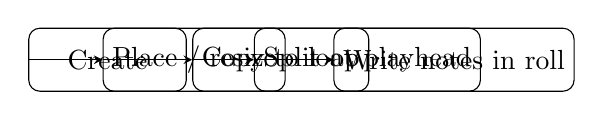
\begin{tikzpicture}[node distance=1.1cm, >=stealth,
    box/.style={draw, rounded corners, align=center, minimum width=2.0cm, minimum height=0.8cm}]
  \node[box] (a) {Create};
  \node[box, right of=a] (b) {Place / resize};
  \node[box, right of=b] (c) {Copy to loop};
  \node[box, right of=c] (d) {Split at playhead};
  \node[box, right of=d] (e) {Write notes in roll};
  \draw[->] (a)--(b); \draw[->] (b)--(c); \draw[->] (c)--(d); \draw[->] (d)--(e);
\end{tikzpicture}
\caption{Common clip flow: create $\to$ place $\to$ copy $\to$ split $\to$ write notes}
\label{fig:ch03-clip-flow}
\end{figure}

\section{Stretch, Merge and Multi-select Editing}

Dragging a clip's edge changes only its time span, not the pitch or relative timing of
its notes (for audio, it changes the playback range). To join adjacent clips into one
continuous piece, align their boundaries first, then merge; the two clips become one
and undo restores them.

With several clips selected, copy, cut and delete apply to the whole group. If only
part of a group is selected, the operation follows the selection and does not touch
unselected clips.

\screenshot{ch03-multi-select}{Three clips selected in the arrangement area with a group-drag preview}

\section{Clip Parameters and the Clip Launch Matrix}

Selecting a clip shows its identity (name, owning track) and editable parameters in
the inspector/clip parameter area. Press Tab to open the \textbf{Clip Launch Matrix}
(Session view): the interface becomes a grid of clips; click a cell to fire that clip,
which suits live launching and improvised arrangements. F5 also switches to Session
view; F6 returns to the Arrangement view.

\screenshot{ch03-clip-matrix}{The Clip Launch Matrix with cells arranged by track, one cell firing}

\section{Cross-track Drag and Track Change}

In the current version, dragging a clip changes only its horizontal position within
the same track. Moving a clip from one track to another is still in evolution
(work item T-FIX-209). So do not treat ``drag onto another track'' as available: to
place material on another track, copy/paste it onto the target track and delete the
original until the capability officially lands. Yeban does not disguise an
unimplemented operation as a success.

\section{Help Topic Mapping}

\begin{table}[htbp]
\centering
\caption{Sections of this chapter $\to$ in-app help anchors}
\label{tab:ch03-help}
\begin{tabular}{ll}
\hline
Section & Help topic \\
\hline
Track types / track header & \texttt{tracks-types-header} \\
Create clips & \texttt{clips-create} \\
Move, resize, cut/copy/paste & \texttt{clips-move-resize} \\
Merge and multi-select editing & \texttt{clips-merge-multiselect} \\
Clip parameters / launch matrix & \texttt{clips-launch-matrix} \\
Cross-track drag and track change & \texttt{clips-cross-track} \\
\hline
\end{tabular}
\end{table}

\paragraph{What you will be able to do} Create the three track types, lay out and cut clips, fire clips from the Launch Matrix, and know which cross-track operations are not yet available.

\paragraph{Hands-on exercise} Create a MIDI synth track and an audio track; create a four-bar MIDI clip, copy it into a two-bar loop and split it at the playhead with Cmd/Ctrl+T; press Tab for Session view and fire a cell; press F6 to return to Arrangement and verify the clips are still there.

% Yeban User Guide — Chapter 4: The Piano Roll (English)
% T-DOC-001 chapter-by-chapter delivery, written ahead of the CH04 task.
% Sources: app.slint roll properties and menus, help.rs tour, bridge.rs pitch lanes,
% docs/manual/04-piano-roll.md, cli.rs SHORTCUTS.

\chapter{The Piano Roll}
\label{ch:piano-roll}

\begin{quote}
凡音之起，由人心生也。
\end{quote}

Source: Book of Rites, “Record of Music” (《礼记·乐记》). Translation: “All music begins in the human heart.”

Before a note lands on the roll there is an emotion to express; technique and rules serve what is heard.

The piano roll is where MIDI notes are written: time runs horizontally, pitch
vertically. This chapter covers opening it, drawing notes, editing velocity and
quantizing, plus the current limits of note dragging.

\section{Open and Navigate the View}

\subsection{Open the roll}

Press P, or switch to the piano roll — the first bottom-console tab; F7 is the direct
key for that tab. Select a clip on a MIDI synth track and the roll shows the notes in
that clip.

\subsection{Read the two dimensions}

The horizontal axis is time (in ticks, converted to bars/beats from the project's time
signature); the vertical axis is pitch, arranged as pitch lanes from high to low, with
key labels on the left (e.g.\ C4, Eb5) as references. A readout at the top shows the
currently visible pitch range. At the bottom is the velocity lane, where each note's
velocity appears as a vertical bar.

\screenshot{ch04-roll-overview}{The piano roll in full, labelling the time ruler, pitch lanes with key labels and the velocity lane}

\subsection{Zoom and framing}

Cmd/Ctrl+Up/Down zooms tracks vertically; Cmd/Ctrl+=/-- zooms the timeline
horizontally. The roll has a "framing" notion: you can frame the current clip, the
current track or all content. Pitches outside the visible window are not drawn —
change the framing to see them.

\section{Note Entry, Selection and Movement}

\subsection{Draw notes}

The onboarding tour puts it plainly: \textbf{number key 2 is the draw tool}; click on
the roll and a note lands there. The drop position comes from the click: horizontal
for time, vertical resolved from the y coordinate into a pitch lane. Once drawn, drag
the note to change time or pitch, or drag its right edge to change length.

\subsection{Select and drag}

Clicking a note selects it. In the current version pointer dragging acts only on the
note under the pointer — even if several are selected, dragging one leaves the others
where they are. So "group drag" and "group duration change" do not work yet; move
notes one at a time, or wait until the capability officially lands. Yeban does not
disguise an unimplemented operation as a success.

\begin{figure}[htbp]
\centering
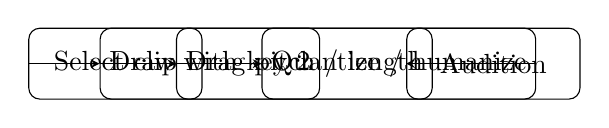
\begin{tikzpicture}[node distance=1.2cm, >=stealth,
    box/.style={draw, rounded corners, align=center, minimum width=2.2cm, minimum height=0.9cm}]
  \node[box] (a) {Select clip};
  \node[box, right of=a] (b) {Draw with key 2};
  \node[box, right of=b] (c) {Drag pitch / length};
  \node[box, right of=c] (d) {Quantize / humanize};
  \node[box, right of=d] (e) {Audition};
  \draw[->] (a)--(b); \draw[->] (b)--(c); \draw[->] (c)--(d); \draw[->] (d)--(e);
\end{tikzpicture}
\caption{Common roll flow: select clip $\to$ draw $\to$ edit pitch/length $\to$ quantize $\to$ audition}
\label{fig:ch04-roll-flow}
\end{figure}

\section{Velocity, Quantize and Scale Tools}

\subsection{Velocity}

In the bottom velocity lane each note has a vertical bar whose height is its velocity.
You can edit a note's velocity directly there; the roll previews the value while
dragging.

\subsection{Quantize and humanize}

Edit $\to$ Note Quantize (Quantize 1/16)... snaps selected notes to a 1/16 grid;
Edit $\to$ Note Humanize... opens a dialog with time jitter, velocity jitter, strength
and seed settings to make mechanical results feel more natural. Both affect only the
current selection.

\screenshot{ch04-humanize-dialog}{The Humanize dialog showing time jitter, velocity jitter and strength inputs}

\subsection{Scale and chord tools}

The current version offers key labels on the pitch lanes as pitch references; whether
standalone scale/chord generation tools exist depends on the build you use — do not
assume an entry that is not present. Edit $\to$ Drum Generation (Drums)... does exist
and can generate a drum clip from style, complexity and seed.

\section{Step Editing and Chord Assistance}

"Step editing" here means writing notes one fixed step at a time: place a note in each
target cell with the draw tool, then use quantize to tidy timing. It is not a
one-click melody generator.

For chords, the available approach is to draw several pitches stacked at the same
moment and verify by ear; automatic chord-progression generation is outside this
chapter's scope and is not described as available.

\section{Help Topic Mapping}

\begin{table}[htbp]
\centering
\caption{Sections of this chapter $\to$ in-app help anchors}
\label{tab:ch04-help}
\begin{tabular}{ll}
\hline
Section & Help topic \\
\hline
Open roll / two dimensions & \texttt{roll-open-view} \\
Zoom and framing & \texttt{roll-zoom-framing} \\
Draw notes and selection & \texttt{roll-note-entry} \\
Select and drag (single-note limit) & \texttt{roll-note-drag} \\
Velocity lane & \texttt{roll-velocity-lane} \\
Quantize and humanize & \texttt{roll-quantize-humanize} \\
Scale tools / step editing & \texttt{roll-scale-step} \\
\hline
\end{tabular}
\end{table}

\paragraph{What you will be able to do} Draw a melody, edit velocity, quantize to 1/16, and explain that dragging currently affects a single note.

\paragraph{Hands-on exercise} Open the roll on a MIDI track clip, draw a one-bar C-major scale with number key 2, make the first note stronger in the velocity lane, quantize with Note Quantize to 1/16, then press Space to audition; finally drag one note and confirm the others stay put.

% Yeban User Guide — Chapter 5: Recording and Audio Editing (English)
% T-DOC-001 chapter-by-chapter delivery, written ahead of the CH05 task.
% Sources: app.slint menus/callbacks, host.rs recording wiring, record_landing.rs,
% docs/manual/03-tracks-clips.md, cli.rs SHORTCUTS.

\chapter{Recording and Audio Editing}
\label{ch:recording-audio}

This chapter covers getting outside sound into a project: recording, importing,
placing audio clips on tracks, and basic trimming and fading. Recorded and imported
material goes into the project's asset pool and travels with it.

\section{Recording Flow and Input Monitoring}

\subsection{Open the record panel}

File $\to$ Record WAV in Real Time... opens the recording panel. It has an Arm switch,
input-device selection and an input test; the recording path uses the project's sample
rate (48 kHz by default). Transport keys are recording-aware: stopping ends the write
rather than quietly carrying on.

\screenshot{ch05-record-panel}{The recording panel with the Arm switch, input-device selection and level monitoring}

\subsection{Where recordings land}

After a successful stop, the bytes land in the project's asset pool with their real
decoded facts (frames, sample rate, channels, bit depth) and, when the wiring is
complete, an ``add clip'' operation is committed to the project — so the recording
appears on the timeline, not only as a WAV on disk. If the current assembly does not
wire the recording write face into the project, the app only writes to disk and does
not pretend a commit happened; that is existing headless/diagnostic behaviour.

\begin{figure}[htbp]
\centering
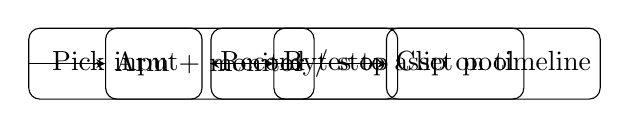
\begin{tikzpicture}[node distance=1.2cm, >=stealth,
    box/.style={draw, rounded corners, align=center, minimum width=2.2cm, minimum height=0.9cm}]
  \node[box] (a) {Pick input};
  \node[box, right of=a] (b) {Arm + monitor};
  \node[box, right of=b] (c) {Record / stop};
  \node[box, right of=c] (d) {Bytes to asset pool};
  \node[box, right of=d] (e) {Clip on timeline};
  \draw[->] (a)--(b); \draw[->] (b)--(c); \draw[->] (c)--(d); \draw[->] (d)--(e);
\end{tikzpicture}
\caption{Recording path: pick input $\to$ arm/monitor $\to$ record/stop $\to$ asset pool $\to$ timeline clip}
\label{fig:ch05-record-flow}
\end{figure}

\section{Audio Clip Trim, Fade In/Out and Crossfade}

\subsection{Import and place}

File $\to$ Import Audio File... reads audio into the project; Track $\to$ Place Latest
Imported Audio on Current Audio Track puts it on the current audio track's timeline.
The landing point follows the playhead and the selected track, so check both before
placing to avoid putting material on the wrong track or at the wrong position.

\subsection{Trim and fade}

Once placed, dragging a clip's left or right edge changes its time span: trimming
leading silence or trailing excess is the most common audio cleanup. A fade-in brings
the head up from silence; a fade-out lets the tail die away; a crossfade across the
overlap of two adjacent clips removes an abrupt seam.

The exact entry points for these operations (clip parameter area, context menu or
Edit menu) depend on the build you use; do not assume a control that is not present.
Fades change only the gain envelope, never the original bytes in the asset pool.

\screenshot{ch05-audio-clip-edges}{An audio clip with draggable left/right edges and fade handles labelled}

\subsection{Don't be misled by a "complete" message}

Stem export measures what was actually rendered and skipped. If every audio clip in a
stem was skipped, the receipt should give the clip-skip count and downgrade the
message rather than still saying merely ``stems complete''. Even when you see
``complete'', cross-check the counts in the receipt (Chapter 8).

\section{The Asset Pool and Audio Asset Management}

Bytes from recording and importing go into the project's asset pool, addressed by
content hash. The direct benefit is a self-contained project: copy the \texttt{.yeban}
file and the sounds it uses travel with the container, so opening it on another
machine does not turn it silent.

\screenshot{ch05-asset-pool}{The asset pool panel listing a project's audio assets and content hashes}

\section{Help Topic Mapping}

\begin{table}[htbp]
\centering
\caption{Sections of this chapter $\to$ in-app help anchors}
\label{tab:ch05-help}
\begin{tabular}{ll}
\hline
Section & Help topic \\
\hline
Record panel / input monitoring & \texttt{record-panel-input} \\
Where recordings land & \texttt{record-landing} \\
Import and place & \texttt{audio-import-place} \\
Trim and fade & \texttt{audio-trim-fade} \\
Don't be misled by ``complete'' & \texttt{audio-receipt-honesty} \\
Asset pool and audio assets & \texttt{audio-asset-pool} \\
\hline
\end{tabular}
\end{table}

\paragraph{What you will be able to do} Record and land a clip on the intended track, import and trim audio, add fades, and verify an export against the receipt.

\paragraph{Hands-on exercise} Create an audio track and put the playhead at 001.01.000; record two bars with Record WAV in Real Time... and stop, verifying the clip appears on the timeline; trim the leading silence and add a fade-out; import another file and place it on a second track with Place Latest Imported Audio...; finally export stems and compare the clip counts in the receipt.

% Yeban User Guide — Chapter 6: Automation and Modulation (English)
% T-DOC-001 chapter-by-chapter delivery, written ahead of the CH06 task.
% Sources: yeban-model/src/project.rs AutomationWriteMode, bridge.rs automation lanes,
% cli.rs SHORTCUTS, yeban-dsp/src/oscillator.rs global LFO, docs/manual/05-mixer-effects.md.

\chapter{Automation and Modulation}
\label{ch:automation-modulation}

\classquote{易穷则变，变则通，通则久。}{Book of Changes, “Appended Judgments II” (《周易·系辞下》)}{Translation: “When a path is exhausted, it changes; through change, it flows; through flow, it endures.” Automation lets parameters change over time; with change, the sound stays alive.}





Automation lets parameters change over time: draw a curve, or record your movements
while playing back. This chapter covers showing lanes, what the four write modes mean,
and the real boundary of modulation in the current build.

\section{Automation Curves and Write Modes}

\subsection{Show the lanes}

Press A in the arrangement area, or use the View automation switch
(Cmd/Ctrl+Shift+A) to show automation lanes. Each non-master track can have its own
lanes, arranged by target parameter. A lane holds a polyline whose vertices are
connected in time order; its horizontal axis aligns with the arrangement timeline, so
you can read the curve directly against clip positions.

\screenshot{ch06-automation-lanes}{Automation lanes expanded in the arrangement area, showing a parameter curve with vertices}

\subsection{Draw and edit the curve}

A lane's polyline is made of vertices. Adding one gives the parameter a value at a
point in time; neighbouring vertices are interpolated. Drag a vertex to change its
time or value; delete one and the curve re-connects across the gap. Curves are saved
with the project, drive parameters during playback and take effect on export too.

\subsection{The four write modes}

Yeban's model defines four automation write modes; knowing them avoids recording
curves you did not mean to:

\begin{description}
  \item[Off] The default. Nothing is written during playback; manual parameter changes do not alter the curve.
  \item[Write] Once the parameter is changed during playback, writing continues until you explicitly stop.
  \item[Touch] Writes only while you are physically touching the parameter; releasing stops immediately. Good for a single corrective nudge.
  \item[Latch] Once touched, writing continues even after you release, until explicitly stopped. Good for locking in a whole fader move.
\end{description}

\begin{table}[htbp]
\centering
\caption{Write modes compared}
\label{tab:ch06-write-modes}
\begin{tabular}{ll}
\hline
Mode & After you release \\
\hline
Off & No writing \\
Write & Keeps writing (explicit stop) \\
Touch & Stops immediately \\
Latch & Keeps writing (explicit stop) \\
\hline
\end{tabular}
\end{table}

\section{Parameter Binding and LFO}

\subsection{Bind a parameter}

An automation lane binds to a specific parameter on a specific track: choose the
target, then draw on that lane. Device parameters (e.g.\ on an insert effect) can also
be automation targets; insert the device, then pick its parameter in the lane's target
list. Parameter changes and automation writes share one commit path, so undo restores
them step by step — you will not get a curve change that the project failed to record.

\subsection{The real LFO boundary}

Yeban's DSP core does implement a \textbf{global LFO} (low-frequency oscillator): one
shared by all voices, evaluated per block, with selectable waveforms. But note
carefully: it is \textbf{not yet wired into the synthesizer's modulation inputs}.
Do not expect to turn an LFO knob in the GUI and get vibrato or filter sweep; those
modulation paths are still evolving.

\begin{figure}[htbp]
\centering
\begin{tikzpicture}[node distance=1.1cm, >=stealth,
    box/.style={draw, rounded corners, align=center, minimum width=2.3cm, minimum height=0.8cm}]
  \node[box] (a) {Pick target};
  \node[box, right=of a] (b) {Pick write mode};
  \node[box, right=of b] (c) {Draw / record};
  \node[box, right=of c] (d) {Playback drives param};
  \node[box, below=of c] (e) {LFO: in DSP, not wired to synth};
  \draw[->] (a)--(b); \draw[->] (b)--(c); \draw[->] (c)--(d);
  \draw[dashed,->] (c)--(e);
\end{tikzpicture}
\caption{Automation flow and the LFO boundary: solid = available path, dashed = modulation not yet wired}
\label{fig:ch06-automation-flow}
\end{figure}

For that reason this chapter does not describe vibrato or filter sweep as available
features. If you cannot find the control in the GUI, it is not wired up yet — you have
not missed it.

\section{Help Topic Mapping}

\begin{table}[htbp]
\centering
\caption{Sections of this chapter $\to$ in-app help anchors}
\label{tab:ch06-help}
\begin{tabular}{ll}
\hline
Section & Help topic \\
\hline
Show the lanes & \texttt{automation-show-lanes} \\
Draw and edit the curve & \texttt{automation-edit-curve} \\
Write modes & \texttt{automation-write-modes} \\
Bind a parameter & \texttt{automation-target-binding} \\
LFO boundary & \texttt{modulation-lfo-boundary} \\
\hline
\end{tabular}
\end{table}

\paragraph{What you will be able to do} Show and edit automation curves, explain Off/Write/Touch/Latch, and know that the LFO exists in the DSP core but is not yet wired into the synthesizer.

\paragraph{Hands-on exercise} Expand an automation lane on a track, select the volume parameter, use Touch mode to nudge the volume while playing and confirm only that touched segment was written; switch back to Off, drag a vertex manually and compare by ear; finally look for an LFO vibrato control and confirm it is not currently provided.

% Yeban User Guide — Chapter 7: Mixer Overview (English)
% T-DOC-001 chapter-by-chapter delivery, written ahead of the CH07 task.
% Sources: app.slint mixer/send/control-room callbacks and menus,
% docs/manual/05-mixer-effects.md, cli.rs SHORTCUTS.

\chapter{Mixer Overview}
\label{ch:mixer-overview}

\begin{quote}
八音克谐，无相夺伦。
\end{quote}

Source: Book of Documents, “Canon of Shun” (《尚书·舜典》). Translation: “Let the eight sounds harmonize, without one usurping another’s place.”

Mixing lets tracks coexist without masking each other; the whole matters more than any single sound.

This chapter follows a signal from a track to the master bus: what a channel strip
holds, in what order inserts take effect, how sends and buses are wired, and where to
watch master monitoring and loudness. Individual effect parameters are out of scope.

\section{Channel Strips and Insert Chains}

\subsection{Open the mixer console}

Press X, or switch to the mixer console in the bottom dock (F8 is also a direct key).
Each track has one channel strip: its volume fader at the top, pan, mute/solo, and the
entry to that track's device chain. All tracks eventually sum into the master bus.

Mix $\to$ Reset Master Fader to 0dB zeroes the master fader in one step — that is a
shortcut for the master bus and does not touch any track fader. The left inspector (I)
shows the same channel-strip details for the selected track; it is the same state as
the mixer, so changes in either place agree.

\screenshot{ch07-mixer-console}{The mixer console in full, labelling channel strips, faders, mute/solo and the master bus}

\subsection{Device chain: instruments first, effects after}

Each track has a device chain: instruments first, effects after, and the order is the
signal-flow order. The bottom Device Rack tab (F9) lets you add/remove devices and
toggle bypass; bypass is per-device and is not the same as deleting a device.

The Track menu can insert three common devices directly into the current track:
Parametric EQ (frequency shaping), Spatial Reverb (a sense of space) and Dynamic
Compressor (taming dynamics, bringing a sound forward). Device parameters can be
automated: expand an automation lane in the arrangement area (A) and parameter-over-
time changes are recorded with the project and applied on export (Chapter 6).

\begin{figure}[htbp]
\centering
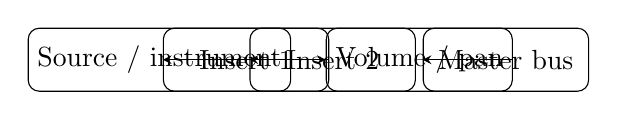
\begin{tikzpicture}[node distance=1.1cm, >=stealth,
    box/.style={draw, rounded corners, align=center, minimum width=2.1cm, minimum height=0.8cm}]
  \node[box] (a) {Source / instrument};
  \node[box, right of=a] (b) {Insert 1};
  \node[box, right of=b] (c) {Insert 2};
  \node[box, right of=c] (d) {Volume / pan};
  \node[box, right of=d] (e) {Master bus};
  \draw[->] (a)--(b); \draw[->] (b)--(c); \draw[->] (c)--(d); \draw[->] (d)--(e);
\end{tikzpicture}
\caption{Signal order: instrument $\to$ inserts (chain order) $\to$ fader/pan $\to$ master bus}
\label{fig:ch07-signal-flow}
\end{figure}

\section{Sends, Buses and the Control Room}

\subsection{Sends and aux buses}

A send routes a copy of one path's signal to another path; an aux bus track (Track
$\to$ New Aux Bus Track) receives those sends for summing or group processing. Sends
can be created and removed from the interface and their gain adjusted; when creation
conditions are not met, the interface states the reason rather than failing silently.

\screenshot{ch07-sends}{The sends area on a channel strip showing destination buses, gain and create/remove entries}

\subsection{Control Room}

Mix $\to$ Show/Hide Control Room (shortcut F4) opens a separate master-monitoring
area: master-bus level and loudness readings, letting you set overall volume without
touching any track fader. It is distinct from the bottom mixer console: the former
governs "what you hear overall", the latter "how each track is balanced".

\screenshot{ch07-control-room}{The Control Room panel showing master-bus level and loudness readings}

\section{Division of Labour with the Mixing Manual}

This chapter is an overview only: where to find controls, roughly how a signal flows,
and how sends and buses are wired. Each effect's parameters, ranges and typical uses
belong to the separate Mixing and Effects manual, which documents them against real
parameter names in the code. The two agree in approach: this chapter says "where",
that volume says "how to adjust".

\section{Help Topic Mapping}

\begin{table}[htbp]
\centering
\caption{Sections of this chapter $\to$ in-app help anchors}
\label{tab:ch07-help}
\begin{tabular}{ll}
\hline
Section & Help topic \\
\hline
Open mixer / channel strip & \texttt{mixer-channel-strip} \\
Insert chain order & \texttt{mixer-insert-chain} \\
Sends and aux buses & \texttt{mixer-sends-buses} \\
Control Room & \texttt{mixer-control-room} \\
Division with the mixing manual & \texttt{mixer-manual-division} \\
\hline
\end{tabular}
\end{table}

\paragraph{What you will be able to do} Find channel strips and the device chain, explain a signal's order, create an aux bus with a send, and know where master monitoring lives.

\paragraph{Hands-on exercise} Press X to open the mixer, insert Parametric EQ on a track and bypass/restore it once from the device rack; create an aux bus track, add a send from the original track and lower its gain; press F4 for the Control Room and read the master-bus level; finally reset the master fader to 0dB and confirm the track faders did not move.

% Yeban User Guide — Chapter 8: Export and Sharing (English)
% T-DOC-001 chapter-by-chapter delivery, written ahead of the CH08 task.
% Sources: app.slint export-dialog properties, docs/manual/06-export.md,
% export_stems.rs (stem receipt and manifest), README.md (CLI entry).

\chapter{Export and Sharing}
\label{ch:export-sharing}

\begin{quote}
既以为人己愈有，既以与人己愈多。
\end{quote}

Source: Laozi, Dao De Jing, ch. 81 (《道德经·第八十一章》). Translation: “The more one gives to others, the more one has; the more one shares, the more one gains.”

Export and sharing hand the work to others; the more you share, the more you gain.

Once a piece is finished it needs to leave Yeban: for mixing elsewhere, for mastering,
or simply as a playable file. This chapter covers what each export route produces and
how to verify the result — the word "complete" alone does not mean it exported right.

\section{WAV Export}

\subsection{Export the full mix}

File $\to$ Export Audio (WAV)... mixes the whole piece into one WAV file. The dialog
offers:

\begin{itemize}
  \item \textbf{Output path}: browse with Ctrl+O.
  \item \textbf{Sample rate}: can be specified; defaults to the project's (shown as \texttt{auto}).
  \item \textbf{Bit depth}: 24 by default.
  \item \textbf{Duration}: in seconds.
  \item \textbf{Bus limiter}: off by default; when on, rendering applies peak limiting on the bus to prevent clipping.
\end{itemize}

\screenshot{ch08-export-wav-dialog}{The Export Audio (WAV) dialog labelling path, sample rate, bit depth, duration and limiter toggle}

\subsection{Read the export receipt}

The export receipt gives measured readings: frame count, true peak and the limiter's
workload, plus the output location. These numbers come from the actual render, not
from copying back the input fields; whether the limiter was on and whether clipping
occurred should be read from the receipt, not guessed.

\section{Stem Export}

\subsection{When to use stems}

File $\to$ Export Stems... renders each source-node track into its own WAV, for mixing
in another program or for mastering. The master bus produces no file but is named in
the skipped list — that is not a dropped track.

Export runs on a background thread so the interface stays responsive; when it finishes
the status message reports how many stems were written, how many skipped and where.
Each stem is a 32-bit Float WAV at the project's sample rate, with a numbered filename
prefix; a \texttt{stems-manifest.json} index in the output directory records each
file's track identity, name, byte count and hash.

\screenshot{ch08-stems-toast}{The stem-export completion message showing written count, skipped count and output directory}

\subsection{Check the receipt, not just "complete"}

The stem receipt starts with a \texttt{exported-stems:} summary line, followed by one
line per stem and per skipped track. Beyond the track-level "skipped" count, look at
the \textbf{audio-clip} dimension: rendered/skipped clip counts. If every audio clip in
a stem was skipped, the message should downgrade to a warning rather than still saying
merely ``stems complete''. When you see ``complete'', cross-checking the clip counts
in the receipt is a good habit.

\begin{figure}[htbp]
\centering
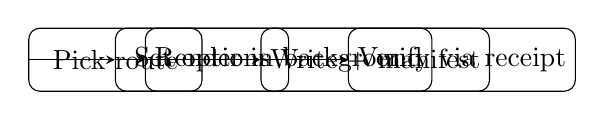
\begin{tikzpicture}[node distance=1.1cm, >=stealth,
    box/.style={draw, rounded corners, align=center, minimum width=2.2cm, minimum height=0.8cm}]
  \node[box] (a) {Pick route};
  \node[box, right of=a] (b) {Set options};
  \node[box, right of=b] (c) {Render in background};
  \node[box, right of=c] (d) {Write + manifest};
  \node[box, right of=d] (e) {Verify via receipt};
  \draw[->] (a)--(b); \draw[->] (b)--(c); \draw[->] (c)--(d); \draw[->] (d)--(e);
\end{tikzpicture}
\caption{Export flow: pick route $\to$ set options $\to$ render $\to$ write $\to$ verify with the receipt}
\label{fig:ch08-export-flow}
\end{figure}

The CLI can export stems too: \texttt{yeban-app --open X.yeban --export-stems stems/};
no window, no MCP session, and the same receipt convention as the GUI.

\section{Project Packaging and Archiving}

The \texttt{.yeban} file is itself the package: tracks, clips, notes, device chains and
the materials they use all live in one container, and saving is atomic (Chapter 2).
So "sharing a project" usually means handing over that file with the assets it
references; the asset pool is addressed by content hash, so opening it elsewhere does
not turn it silent.

Diagnostics $\to$ Export Project Diagnostic Bundle produces a troubleshooting bundle,
not artwork audio; attach it when asking someone to look at a broken project.

\section{Help Topic Mapping}

\begin{table}[htbp]
\centering
\caption{Sections of this chapter $\to$ in-app help anchors}
\label{tab:ch08-help}
\begin{tabular}{ll}
\hline
Section & Help topic \\
\hline
Full mix / dialog options & \texttt{export-wav-dialog} \\
Read the WAV receipt & \texttt{export-wav-receipt} \\
When to use stems & \texttt{export-stems-purpose} \\
Check the receipt, not just ``complete'' & \texttt{export-stems-receipt} \\
Project packaging and archiving & \texttt{export-project-archive} \\
\hline
\end{tabular}
\end{table}

\paragraph{What you will be able to do} Pick the right export route, set dialog options, verify output with the receipt (including clip counts), and know that a diagnostic bundle is not the piece.

\paragraph{Hands-on exercise} Export a full-mix WAV with the limiter on and read the frame count and true peak in the receipt; then export stems, check file names and byte counts against \texttt{stems-manifest.json}, and find the rendered/skipped audio-clip counts in the receipt; finally export stems for the same project from the CLI and compare the audio samples from both routes.

% Yeban User Guide — Chapter 9: Shortcuts and Command Reference (English)
% T-DOC-001 chapter-by-chapter delivery, written ahead of the CH09 task.
% Sources: cli.rs SHORTCUTS (the single authoritative table), help.rs in-app reference,
% docs/manual/README.md writing rule (no second hand-copied key table).

\chapter{Shortcuts and Command Reference}
\label{ch:shortcuts}

\begin{quote}
以无厚入有间，恢恢乎其于游刃必有余地矣。
\end{quote}

Source: Zhuangzi, “The Secret of Caring for Life” (《庄子·养生主》). Translation: “Where there is no thickness to enter what has gaps, there is ample room for the blade to move.”

Shortcuts make frequent actions effortless; once the hands know the way, the mind can stay with the music.

Yeban has a single authoritative shortcut policy table: the one shown under Help $\to$
Shortcuts, which is the same table printed by \texttt{yeban-app --print-shortcuts}.
This chapter groups common keys by workflow as a memory aid; it is not a second
authoritative table — for the full list and implementation status, use the in-app
reference.

\section{The Policy Table Shared with In-app Help}

\subsection{Why this chapter does not copy the full table}

The policy table evolves: it marks row by row which keys are implemented and which are
"bound but not yet implemented" in the host. A hand-copied table goes stale quickly and
can turn "not implemented" into "available". So this chapter does only two things:
explain the canonical key notation, and pick out high-frequency operations by workflow.

\subsection{Canonical notation and platform folding}

The table keeps the cross-platform canonical form \texttt{Cmd/Ctrl+}: on macOS it
renders as \texttt{Cmd+}, elsewhere as \texttt{Ctrl+}. So \texttt{Ctrl+S} on Windows
and \texttt{Cmd+S} on macOS are the same canonical binding. A key marked "(not
implemented)" is bound and resolves to an action, but the host has no implementation
yet and rejects the press — the key is not broken.

\section{Common Keys by Workflow}

The keys below all come from the policy table, grouped in the order you tend to work.

\subsection{Projects and editing}

\begin{description}
  \item[Cmd/Ctrl+N] New MIDI synth track.
  \item[Cmd/Ctrl+O] Open project.
  \item[Cmd/Ctrl+S] Save project; Cmd/Ctrl+Shift+S save as.
  \item[Cmd/Ctrl+Z] Undo; Cmd/Ctrl+Shift+Z redo.
  \item[Tab] View switch (canvas focus only); F5 Session view, F6 Arrangement view.
\end{description}

\subsection{Arranging and editing clips}

\begin{description}
  \item[Space] Play/pause; Shift+Space resume from cursor.
  \item[Enter] Return to start; C cycle playback toggle.
  \item[Cmd/Ctrl+T] Split selected clip at the playhead.
  \item[Cmd/Ctrl+C / V / X] Copy / paste / cut clips.
  \item[Cmd/Ctrl+= / -] Zoom the timeline horizontally in/out.
  \item[Cmd/Ctrl+Up/Down] Zoom tracks vertically out/in.
\end{description}

\subsection{Bottom console and panels}

\begin{description}
  \item[P / F7] Piano roll; X / F8 mixer console; F9 device rack; F3 console device stack.
  \item[I] Toggle the left inspector.
  \item[Cmd/Ctrl+Shift+A] Show automation lanes.
  \item[Cmd/Ctrl+Shift+B] Open the unified browser (sounds/samples/presets/effects).
  \item[E] Toggle editor view.
\end{description}

\subsection{Recording and other}

\begin{description}
  \item[R] Recording on/off.
  \item[Cmd/Ctrl+Shift+H] Time Machine.
  \item[Esc] Close the command palette / hotspot overlay.
\end{description}

\subsection{The IME exception}

In text input and IME composition mode, every key except F5/F6 is swallowed by the
input method and does not trigger the actions above — deliberately, so typing does not
fire shortcuts. The policy table has separate columns explaining "canvas focus"
versus "text input + IME composition".

\screenshot{ch09-shortcuts-panel}{The Help $\to$ Shortcuts panel showing canonical form, keys, actions and implementation status columns}

\begin{figure}[htbp]
\centering
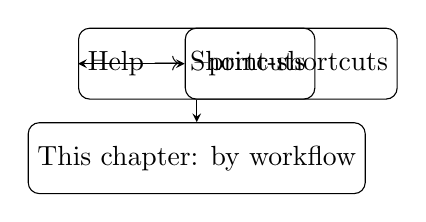
\begin{tikzpicture}[node distance=1.2cm, >=stealth,
    box/.style={draw, rounded corners, align=center, minimum width=2.2cm, minimum height=0.9cm}]
  \node[box] (a) {Help $\to$ Shortcuts};
  \node[box, right of=a] (b) {--print-shortcuts};
  \node[box, below of=a] (c) {This chapter: by workflow};
  \draw[<->] (a)--(b); \draw[->] (a)--(c);
\end{tikzpicture}
\caption{The authoritative source is the one policy table behind the in-app reference and \texttt{--print-shortcuts}; this chapter is only a guide}
\label{fig:ch09-shortcut-source}
\end{figure}

\section{Help Topic Mapping}

\begin{table}[htbp]
\centering
\caption{Sections of this chapter $\to$ in-app help anchors}
\label{tab:ch09-help}
\begin{tabular}{ll}
\hline
Section & Help topic \\
\hline
Shared policy table / notation & \texttt{shortcuts-policy-table} \\
Projects and editing & \texttt{shortcuts-project-edit} \\
Arranging and clips & \texttt{shortcuts-arrange} \\
Console and panels & \texttt{shortcuts-panels} \\
Recording and other & \texttt{shortcuts-record-misc} \\
IME exception & \texttt{shortcuts-ime-exception} \\
\hline
\end{tabular}
\end{table}

\paragraph{What you will be able to do} Find high-frequency keys by workflow, understand the \texttt{Cmd/Ctrl+} platform folding, and know that the full list lives in the in-app reference, not this chapter.

\paragraph{Hands-on exercise} Open Help $\to$ Shortcuts and pick three keys from this chapter that you use often but know less well; run \texttt{yeban-app --print-shortcuts} and confirm it shows the same bindings; finally, using only the keyboard, do "open project $\to$ split a clip $\to$ save".

% Yeban User Guide — Chapter 10: Terminal and Automation Entry Points (English)
% T-DOC-001 chapter-by-chapter delivery, written ahead of the CH10 task.
% Sources: README.md, docs/README.md, docs/tool-availability.md,
% presence of crates/yeban-tui, cli.rs switches. Tool counts are never hand-copied.

\chapter{Terminal and Automation Entry Points}
\label{ch:entry-points}

\classquote{天下同归而殊涂，一致而百虑。}{Book of Changes, “Appended Judgments II” (《周易·系辞下》)}{Translation: “All beneath heaven returns to one end though the roads differ; all reaches one goal though thoughts are many.” The GUI, the terminal, and MCP are different entries into the same project.}





The same project can be operated through three entry points: the desktop GUI, a
terminal TUI and the command line CLI, plus an MCP tool surface for AI agents. They
share one project model and backend, so they do the same work with different
interaction styles. This chapter gives one section each and says when to use which.

\section{TUI}

Yeban provides a terminal user interface (TUI) entry point, with source in
\texttt{crates/yeban-tui}. It serves setups without a graphical desktop, or users who
prefer working in a terminal, without opening a window; the panels and keys it actually
offers are documented by that entry point's own help, not hand-copied here where they
could go stale.

\begin{table}[htbp]
\centering
\caption{What each entry point suits}
\label{tab:ch10-entry-compare}
\begin{tabular}{ll}
\hline
Entry & Best for \\
\hline
Desktop GUI & Everyday arranging, notes, mixing, visual feedback \\
TUI & Terminal environments, no graphical desktop, remote shells \\
CLI & Batch work, scripts, export, CI \\
MCP & AI agents editing and querying through tool calls \\
\hline
\end{tabular}
\end{table}

\section{CLI}

\subsection{Read the help first}

The complete switch list and exit codes come from \texttt{yeban-app --help}; this
chapter is a guide, not a replacement. Common entries:

\begin{description}
  \item[\texttt{--open <path>}] Open a given project directly (GUI or batch).
  \item[\texttt{--export-wav}] Export the full mix; pair with \texttt{--loudness-target} and \texttt{--true-peak-ceiling} for mastering. An unreachable target fails loudly rather than silently degrading.
  \item[\texttt{--export-stems <dir>}] Export stems with the same backend as the MCP tool; track-selection switches can limit it to named tracks.
  \item[\texttt{--apply-ops}] Commit a file of edit operations as one batch.
  \item[\texttt{--export-song-overview}] Export the whole-song overview (energy/frequency/density/emotion with an anomaly summary).
  \item[\texttt{--print-shortcuts}] Print the shortcut policy table (the same source as the GUI's Help $\to$ Shortcuts).
  \item[\texttt{--headless}] Run on a machine without a display.
\end{description}

\subsection{Know the feature gates}

Some switches are gated by build features. In a default build the MCP-related
\texttt{in-process-mcp} is on — but "compiled in" is not "listening": at runtime you
still need \texttt{--enable-mcp-http} or the environment variable
\texttt{YEBAN\_MCP\_HTTP=1}. With \texttt{--no-default-features}, calling a gated
switch yields a usage error naming the feature (exit code 2), never a silent ignore.
Experimental exports such as \texttt{--export-als} and \texttt{--export-logic} are off
by default and only compile when requested.

\section{MCP}

\subsection{Two forms, one registry}

MCP has two forms sharing a single \texttt{TOOLS} registry and the same domain
implementation:

\begin{description}
  \item[Form A (library form)] Hosted in-process by \texttt{yeban-app}, for an AI agent working on a running DAW; transport is loopback HTTP (\textbf{only} \texttt{127.0.0.1}) or direct in-process calls.
  \item[Form B (binary form)] A standalone \texttt{yeban-mcp} binary over stdio for batch work without a GUI.
\end{description}

Network listening binds only the loopback address, never \texttt{0.0.0.0} — a safety
red line. \texttt{yeban-mcp}'s own \texttt{mcp-http} is never in its default features;
only the host can forward-enable it.

\screenshot{ch10-mcp-modes}{The two MCP forms: in-app mount over loopback HTTP, standalone binary over stdio}

\begin{figure}[htbp]
\centering
\begin{tikzpicture}[node distance=1.2cm, >=stealth,
    box/.style={draw, rounded corners, align=center, minimum width=2.4cm, minimum height=0.9cm}]
  \node[box] (a) {One TOOLS registry};
  \node[box, below left=of a] (b) {Form A: in-app mount};
  \node[box, below right=of a] (c) {Form B: standalone binary};
  \node[box, below=of b] (d) {Loopback HTTP 127.0.0.1};
  \node[box, below=of c] (e) {stdio batch};
  \draw[->] (a)--(b); \draw[->] (a)--(c); \draw[->] (b)--(d); \draw[->] (c)--(e);
\end{tikzpicture}
\caption{Both MCP forms share one registry; network listening binds only loopback}
\label{fig:ch10-mcp-forms}
\end{figure}

\subsection{Don't trust hand-copied tool counts}

The tool count must be read live from the three constants in
\texttt{crates/yeban-mcp/src/tools.rs} and the enum in
\texttt{schemas/mcp-tools.schema.json}: numbers in documentation have gone stale
repeatedly and old manuals disagree with each other. This chapter deliberately gives
no concrete number.

Some tools depend on a provider injected by the host (e.g.\ an external SVS singing
service). Form B has no injector, so calling such a tool returns the
\texttt{providerUnavailable} contract rather than pretending success.

\section{Help Topic Mapping}

\begin{table}[htbp]
\centering
\caption{Sections of this chapter $\to$ in-app help anchors}
\label{tab:ch10-help}
\begin{tabular}{ll}
\hline
Section & Help topic \\
\hline
TUI & \texttt{entry-tui} \\
CLI: help / common switches & \texttt{entry-cli-switches} \\
CLI: feature gates & \texttt{entry-cli-features} \\
MCP: two forms & \texttt{entry-mcp-forms} \\
MCP: tool counts and providers & \texttt{entry-mcp-tools} \\
\hline
\end{tabular}
\end{table}

\paragraph{What you will be able to do} Pick the right entry for the situation, know common CLI switches and feature gates, and explain that both MCP forms share one registry while network listening binds only loopback.

\paragraph{Hands-on exercise} Use \texttt{yeban-app --help} to find the exact stem-export switch, export stems from both the GUI and CLI for the same project and compare receipts; run \texttt{yeban-app --print-shortcuts} against the GUI panel; finally confirm that without \texttt{--enable-mcp-http} the MCP HTTP port is not listening.

% Yeban User Guide — Chapter 11: Troubleshooting (English)
% T-DOC-001 chapter-by-chapter delivery, written ahead of the CH11 task (last outline chapter).
% Sources: docs/manual chapters, AGENTS.md execution discipline, T-FIX-196 memory threshold,
% app.slint device/diagnostic entries.

\chapter{Troubleshooting}
\label{ch:troubleshooting}

\begin{quote}
人谁无过？过而能改，善莫大焉。
\end{quote}

Source: Zuo Zhuan, 2nd year of Duke Xuan (《左传·宣公二年》). Translation: “Who among us has no faults? To err and be able to change is the greatest good.”

Mistakes are not the end: follow the clues, correct the cause, and the project moves on.

This chapter is organised by symptom: what you see, then what to rule out. Each section
moves from the most likely and easiest-to-check cause towards project and device levels;
change one thing at a time and audition after each. One guiding rule throughout: Yeban
records key facts in receipts and the status bar — do not conclude from "it looks fine".

\section{No Sound}

Work through these in order, changing only one thing per step and listening after each:

\begin{enumerate}
  \item \textbf{Transport and playhead}: is playback actually running? Press Space and watch the playhead advance; Shift+Space resumes from the cursor.
  \item \textbf{Mute / solo}: are Mute or Solo engaged on the track header or in the mixer? If another track is soloed, the current one is silent by design.
  \item \textbf{Fader and pan}: is the track fader or master fader all the way down? Mix $\to$ Reset Master Fader to 0dB restores the master in one step.
  \item \textbf{Device chain}: did the instrument load? Is an effect bypassed? Bypassed devices are not the same as deleted ones.
  \item \textbf{Clip and fades}: is there actually a clip under the playhead? Was it trimmed down to silence, or are its fade-in/fade-out swallowing the whole thing?
  \item \textbf{Materials present?}: a missing embedded sample is recorded as MissingSample and the track is skipped (saving still succeeds). Check the asset pool for the audio it uses; relative SFZ paths depend on the project directory — a project opened from file uses the real directory, while an unsaved new project uses a placeholder under the output directory, which breaks samples kept only next to the project file.
  \item \textbf{Control Room}: does the master-bus meter show a level? Level present but nothing heard points to the output device; no level points to the project side.
\end{enumerate}

\screenshot{ch11-silence-checklist}{The silence checklist as presented in the help panel}

\section{Devices and Drivers}

\subsection{Input device and level}

The recording panel has input-device selection and an input test, so you can confirm a
signal arrives before actually recording. The recording path uses the project's sample
rate (48 kHz by default); after changing devices, the next recording uses the new one.

\subsection{Output and latency}

If the project-side meter shows level but you hear nothing, check the system output
device and the Control Room's master-bus reading. Yeban targets low-latency
determinism and handles internal plug-in delay compensation; for latency-sensitive
work, check the device buffer settings first rather than hunting for interface switches.

\subsection{Safe defaults}

Network-listening services (MCP HTTP) bind only the loopback address \texttt{127.0.0.1},
never \texttt{0.0.0.0}; a default build does not listen at all unless you explicitly pass
\texttt{--enable-mcp-http} or set \texttt{YEBAN\_MCP\_HTTP=1}. If MCP "won't connect" and
you are tempted to open up listening, check that runtime switch first — do not change
the bind address.

\section{A Project Will Not Open}

\begin{enumerate}
  \item \textbf{Check the file}: \texttt{.yeban} is the only project format. Saving is atomic, so a power cut mid-write usually leaves the previous complete version rather than half a file; try a backup if you have one.
  \item \textbf{Use the right entry}: File $\to$ Open / Restore Project..., or \texttt{yeban-app --open <path>}; the startup chooser's Recent Projects tab also returns you to prior work.
  \item \textbf{Are the assets alongside it?}: the project references asset-pool materials by content hash. If you copied only the \texttt{.yeban} file and lost referenced materials, the project opens but those tracks are silent — that is not "won't open".
  \item \textbf{Export a diagnostic bundle}: Diagnostics $\to$ Export Project Diagnostic Bundle produces a troubleshooting bundle (not artwork audio). Attaching it is far more useful than a vague description when asking for help.
  \item \textbf{Record errors verbatim}: if the app reports an error code or a missing list, note the original text; do not substitute "it looks like the same problem as last time" for a measurement.
\end{enumerate}

\section{Performance and Memory Thresholds}

\subsection{Know the threshold}

The app test target is heavy: measured on a 4 GB machine, \texttt{cargo test -p yeban-app}
is killed by the kernel (rustc SIGKILL) at roughly 35 minutes, yielding no results; moving
the same kind of assertions into a lighter crate (\texttt{yeban-model}) compiled in about
1m39s and ran in about 1s. The practical threshold for app-side verification is at least
8 GB; below it, app-side work can only be static changes — do not claim tests were run.

\subsection{A minimum verification set when resources are tight}

When memory is insufficient, use the smallest set you can actually complete:
\texttt{cargo fmt --check}, \texttt{cargo check --all-targets} and clippy for the target
crate. Record what could not run honestly as \texttt{not\_run} with the reason, and let CI
rerun it on a larger machine. For building, use
\texttt{cargo build --profile release-small -p yeban-app}; on a headless machine add
\texttt{--headless}.

\subsection{Only the CI verdict counts}

A local green is only a reference; the final verdict belongs to CI. An unread verdict
counts as pending, never as "passed". Also avoid treating an overall "success" as proof
that the target assertions actually ran — confirm the job executed (non-zero duration)
and its log contains test-result lines.

\section{Help Topic Mapping}

\begin{table}[htbp]
\centering
\caption{Sections of this chapter $\to$ in-app help anchors}
\label{tab:ch11-help}
\begin{tabular}{ll}
\hline
Section & Help topic \\
\hline
No sound & \texttt{troubleshoot-silence} \\
Devices and drivers & \texttt{troubleshoot-devices} \\
A project will not open & \texttt{troubleshoot-project-open} \\
Performance and memory thresholds & \texttt{troubleshoot-performance} \\
Minimum verification and CI verdict & \texttt{troubleshoot-verification} \\
\hline
\end{tabular}
\end{table}

\paragraph{What you will be able to do} Work through silence, device and project-open failures symptom by symptom, know the 8 GB threshold and the minimum verification set, and understand that the CI verdict is final.

\paragraph{Hands-on exercise} Reproduce "no sound": mute a track then unmute it, bypass then restore an effect, auditioning after each step and naming which step restored sound; then export a diagnostic bundle and confirm it is a diagnostic file, not the piece; finally run the minimum verification set in a low-memory environment and record the unrunnable items honestly as \texttt{not\_run}.

\printindex
\end{document}
